\documentclass{article}

\usepackage{amsmath}
\usepackage{graphicx}

\def\I{\overline{I}}
\def\d{\mathrm{d}}
\def\x{\vec{x}}
\def\vnu{\vec{\nu}_{m,n}}
\def\nuth{\nu_{m,n|\theta}}
\def\ui{\hat{\imath}}
\def\uj{\hat{\jmath}}
\def\real{\mathrm{Re}}
\def\imag{\mathrm{Im}}

\title{A Brief Derivation for Spatial DFT Extraction from Langmuir Probe Currents}
\author{Christopher R. Martin\\Associate Professor of Mechanical Engineering\\Penn State Altoona}
\date{\today}

\begin{document}

\maketitle

\section{Derivation}

The probe wire has radius, $R$, and rotates about a center on the $x$-axis a distance, $d$, from the origin.  At each sample, the probe will have an angle, $\theta$, will enter the domain at radius, $R_0$, and terminates at a radius, $R_1$.  The current measured by the probe, $I$, is an integral of the current per unit wire length, $\I$,
\begin{align}
I = \int_{R_0}^{R_1} \I \d r.
\end{align}
These dimensions are shown in Figure \ref{fig:coords}.  When the tip of the wire lies inside the domain, $R_1 = R$.

\begin{figure}
\centering
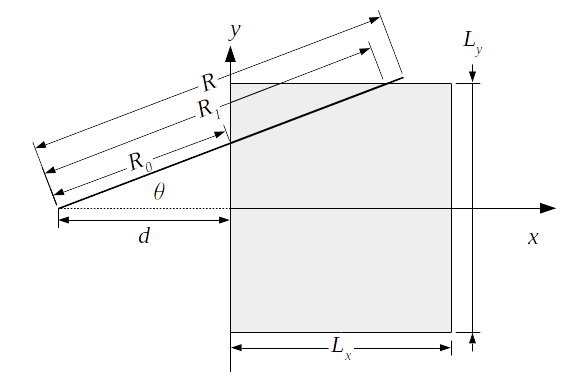
\includegraphics[width=.9\linewidth]{figures/coords}
\caption{Dimensions and coordinate system for the domain}\label{fig:coords}
\end{figure}

The wire current density is a function of the bulk velocity and the ion density, so it is expressed as a function of position in the fluid, $\I(\x)$.  Once $\I(\x)$ is known everywhere in the fluid, it is be possible to calculate the ion density distribution.  

Previously, wire current density was calculated as a grid of discrete nodes, and its integral along the wire length was calculated by interpolating along its path.  This approach is intuitive and flexible, and the inversion problem results in a sparse symmetrical matrix, which can speed inversion times.  On the other hand, the path tracing algorithm required iteration along the wire's length, which is slow in high-level languages, the discretization scheme produces artifacts in the images, and there were also unexplained striping artifacts in the wake of strong signals.

In the present work, we adopt a spatial Fourier series, which provides a far more numerically elegant formulation.

\subsection{Fourier series}

The Fourier series for $\I$ is constructed in $x,y$ coordinates
\begin{align}
\I(x,y) &= \sum_{m=-N_x}^{N_x} \sum_{n=-N_y}^{N_y} c_{m,n} \exp\left(2\pi j \vnu \cdot \x \right),\label{eqn:Ibar}
\end{align}
where $\vnu$ is the wavenumber vector,
\begin{align}
\vnu = \frac{m}{N_x L_x} \ui + \frac{n}{N_y L_y} \uj,
\end{align}
and $\x$ is the position in the domain,
\begin{align}
\x = x \ui + y \uj.
\end{align}

This formulation has $(2N_x+1)(2N_y+1)$ complex coefficients, and represents a function with periodicity $L_x$ on $x$ and $L_y$ on $y$.  It is continuous, but cannot resolve features with wavelengths shorter than $L_x / N_x$ and $L_y / N_y$.  In this way, the results are effectively spatially filtered by the highest wavenumber in the expansion.

Because the coefficients are complex-valued, each of the $(2N_x+1)(2N_y+1)$ coefficients represents two unknowns.  However, because the function, $\I$, is strictly real-valued, the coefficients must occur in complex conjugate pairs.  As we will examine in more depth later, the number of unknonws only scales like $4N^2$ (when $N = N_x = N_y$)

\subsection{Evaluating the integral}

The integral of $\I$ requires an $x,y$ parametric formulation of the wire's path.  At an angle, $\theta$, the wire is oriented along a unit vector,
\begin{align}
\hat{e}_\theta = \cos(\theta) \ui + \sin(\theta) \uj.
\end{align}


If $r$ is the distance along the wire from the disc center, the corresponding location in $(x,y)$ is
\begin{align}
\x &= r \hat{e}_\theta - d \ui
\end{align}
The wavenumber along the wire (in the $\hat{e}_\theta$ direction) can be written as a scalar,
\begin{align}
\nuth &= \vnu \cdot \hat{e}_\theta\nonumber\\
 &= \frac{m}{L_x} \cos(\theta) + \frac{n}{L_y} \sin(\theta).
\end{align}

The radius at which the wire crosses into the domain, $R_0$, the radius at which the wire either terminates or leaves the domain, $R_1$, and the wire length in the domain, $\Delta R$, are
\begin{align}
R_0 &= \frac{d}{c_\theta}\\
R_1 &= \min\left(\ R,\ \frac{d + L_x}{\cos(\theta)},\ \left|\frac{L_y}{2\sin(\theta)}\right|\ \right)
\end{align}
The integral is a sum of surface currents along the wire's length at moment in time, so the disc position parameters, $d$ and $\theta$, are constant.  For compactness of notation, it will become convenient to express the trigonometric functions on $\theta$ as constants, $c_\theta$ and $s_\theta$.

A single term of the Fourier series appears
\begin{align*}
&c_{m,n} \exp\left(2\pi j \vnu \cdot \x \right)\\
&\hspace{2em}= c_{m,n} \exp\left(2\pi j \vnu \cdot (\hat{e}_\theta r - d \ui) \right)\\
&\hspace{2em}= c_{m,n} \exp\left(-2\pi j \frac{md}{L_x} \right) \exp\left(2\pi j \nuth r \right)
\end{align*}


For an integral over $r$, all but the last portion of the term above is constant, so it is convenient to define a new parameter, $\gamma$, which represents the value of this term integrated over $r$:
\begin{align}
\gamma_{m,n}(d,\theta) &= \int_{R_0}^{R_1} \exp\left(2\pi j \nuth r \right) \d r \nonumber\\
 &= \left\{\begin{array}{c|l}
 R_1 - R_0 & \nuth = 0\\
 \left.\frac{1}{2\pi j \nuth}\exp\left(2\pi j \nuth r \right)\right|^{R_1}_{R_0} & \mathrm{otherwise}
\end{array}
\right.
\end{align}
The wavenumber, $\nuth$, can be zero when $m=n=0$ or when $\x$ is exactly normal to the wavenumber vector.

This yields an expression for the total wire current
\begin{align}
I(d,\theta) &= \sum_{m=-N_x}^{N_x} \exp\left(-2\pi j \frac{md}{L_x} \right) \sum_{n=-N_y}^{N_y} c_{m,n} \gamma_{m,n}(d,\theta)
\end{align}

\subsection{Offset current}

Every experiment begins by zeroing the current signal to the nearest practical precision, but no real signal will ever be perfectly zero to numerical precision.  Normally, this would not be especially problematic, but the derivation above provides no representation of current sources outside of the domain.  To prevent the kinds of bizarre numerical phenomena that can occur when models awkwardly attempt to match behaviors beyond their capability, it is prudent to add a global offset parameter, $I_0$,  
\begin{align}
I(d,\theta) &= I_0 + \sum_{m=-N_x}^{N_x} \exp\left(-2\pi j \frac{md}{L_x} \right) \sum_{n=-N_y}^{N_y} c_{m,n}\gamma_{m,n}\label{eqn:I}.
\end{align}

\subsection{Alternate realization}

Because the $c_{m,n}$ coefficients must occur in complex conjugate pairs, half of the $2(2N_x+1)(2N_y+1)$ unknown values represent redundant information.  The current density formulation in Equation \ref{eqn:Ibar} can be reorganized around complex conjugates:
\begin{align}
I(d,\theta) &= c_{0,0} \nonumber\\
& \hspace{-1em} + \sum_{n=1}^{N_y} c_{0,n} \exp(2\pi j \vec{\nu}_{0,n} \cdot \x) + c_{0,n}^* \exp(-2\pi j \vec{\nu}_{0,n} \cdot \x)\nonumber\\
& \hspace{-1em} + \sum_{m=1}^{N_x}\sum_{n=-N_y}^{N_y} c_{m,n} \exp(2\pi j \vec{\nu}_{m,n} \cdot \x) + c_{m,n}^* \exp(-2\pi j \vec{\nu}_{m,n} \cdot \x).
\end{align}
This works because $\vec{\nu}_{-m,-n} = -\vnu$, and so $c_{-m,-n} = c_{m,n}^*$.  Figure \ref{fig:wavenumbers} shows these complimentary wavenumber vectors in the wavenumber plane.  The grouped terms above are shown in green blocks with their omitted complimentary terms in red.  This is probably the simplest way to show why three terms are necessary: if the domain were expressed using only one sum, the $(-m,-n)$ pair would incorrectly repeat terms at the origin and along the $\nu_y$-axis.  

\begin{figure}
\centering
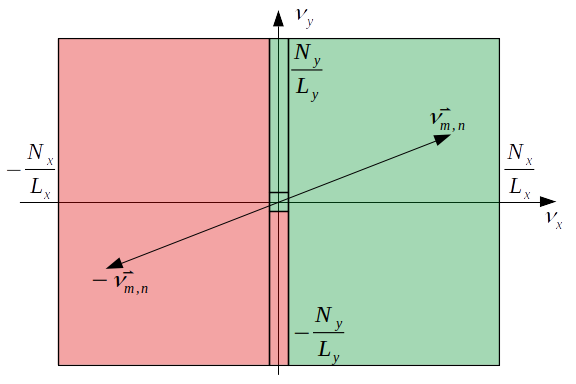
\includegraphics[width=0.9\linewidth]{figures/wavenumbers}
\caption{The wave number space with the included terms marked in green and their negative mirrors marked in red.}\label{fig:wavenumbers}
\end{figure}

The choice to select the $\nu_y$-axis as the line about which to mirror the domain is arbitrary.  It is equally valid to split the domain by the $\nu_x$-axis, or any line passing through the origin.  It is even possible to disperse points quasi-randomly, but there is no clear benefit to such a scheme.

Once grouped into conjugates, these terms yield
\begin{align}
I(d,\theta) &= a_{0,0} \nonumber\\
& \hspace{-1em} + \sum_{n=1}^{N_y} a_{0,n} \cos(2\pi \vec{\nu}_{0,n} \cdot \x) + b_{0,n} \sin(2\pi \vec{\nu}_{0,n} \cdot \x)\nonumber\\
& \hspace{-1em} + \sum_{m=1}^{N_x}\sum_{n=-N_y}^{N_y} a_{m,n} \cos(2\pi j \vec{\nu}_{m,n} \cdot \x) + b_{m,n} \sin(2\pi j \vec{\nu}_{m,n} \cdot \x).
\end{align}
when
\begin{align}
a_{m,n} &= \left\{\begin{array}{c|l}
c_{0,0} & m=n=0\\
c_{m,n} + c_{m,n}^*& \mathrm{otherwise}
\end{array}\right.\\
b_{m,n} &= \left\{\begin{array}{c|l}
0 & m=n=0\\
-j(c_{m,n} - c_{m,n}^*) & \mathrm{otherwise}
\end{array}\right.
\end{align}

\section{Inversion}

Fourier transforms classically take advantage of the orthogonality of the sinusoidal basis functions, so the original signal only needs to be integrated against each basis function over the entire domain to calculate the magnitude and phase of that component.  Because no single wire position spans the entire domain, this approach is not tenable.  Instead, a vector of coefficients must be solved by inverting a matrix.

The exact scheme used to organize the coefficients into a vector, $\vec{c}$, is not especially important, but it might be something along the lines of 
\begin{align}
\vec{c} = [I_0,\ c_{0,0},\ c_{1,0},\ \ldots ]^T.
\end{align}
As we show in the previous seciton, it is equally valid to express the problem in terms of a purely real vector constructed from the coefficients of sines and cosines,
\begin{align}
\vec{d} = [I_0,\ a_{0,0},\ a_{1,0},\ \ldots\ b_{0,0},\ b_{1,0},\ \ldots]^T.
\end{align}

If the coefficients of these vectors were arranged into groups, they are related by a convenient linear transforms,
\begin{align}
\vec{d} = \left[\begin{array}{c}
I_0\\
a_{0,0}\\
\vec{a}\\
\vec{b}
\end{array}\right] &= 
\left[\begin{array}{cccc}
1 & 0 & 0 & 0\\
0 & 1 & 0 & 0\\
0 & 0 & \mathbf{I} & \mathbf{I}\\
0 & 0 & -j\mathbf{I} & -j\mathbf{I}
\end{array}\right]
\left[\begin{array}{c}
I_0\\
c_{0,0}\\
\vec{c}\,^+\\
\vec{c}\,^-
\end{array}\right] = \mathbf{P} \vec{c}\\
\vec{c} = \left[\begin{array}{c}
I_0\\
c_{0,0}\\
\vec{c}\,^+\\
\vec{c}\,^-
\end{array}\right] &= 
\left[\begin{array}{cccc}
1 & 0 & 0 & 0\\
0 & 1 & 0 & 0\\
0 & 0 & \frac{1}{2} \mathbf{I} & \frac{j}{2} \mathbf{I}\\
0 & 0 & \frac{1}{2} \mathbf{I} & -\frac{j}{2} \mathbf{I}
\end{array}\right]
\left[\begin{array}{c}
I_0\\
a_{0,0}\\
\vec{a}\\
\vec{b}
\end{array}\right] = \mathbf{P}^{-1} \vec{d}
\end{align}

When the terms of (\ref{eqn:I}) are embedded into a second vector, $\vec{\Lambda}$, the equation may be rewritten
\begin{align}
I(d,\theta) = \vec{\Lambda}(d,\theta) \cdot \vec{x}.
\end{align}
Here, $\vec{\Lambda}$, is a vector that models the contribution of each coefficient to the current of a wire in location $(d,\theta)$.

For a given wire position, $(d_i, \theta_i)$, there will be a measured current, $I_i$.  For a given coefficient set, there will be an error,
\begin{align}
e_i = I_i - \vec{\Lambda}(d_i, \theta_i) \cdot \vec{x}.
\end{align}
In a least squares approach, we differentiate the sum of the squares of errors for each of the data points.  For compactness of notation, it will be convenient to abbreviate $\vec{\Lambda}_i = \vec{\Lambda}(d_i, \theta_i)$ moving forward.

\begin{align}
\vec{0} = \nabla \sum e_i {^2} = \sum 2(I_i - \vec{\Lambda}_i \cdot \vec{x})(- \vec{\Lambda}_i)
\end{align}
Solving for $\vec{x}$,
\begin{align}
\vec{x} = \left(\sum \vec{\Lambda}_i \vec{\Lambda}_i{^T}\right)^{-1} \sum I_i \vec{\Lambda}_i
\end{align}

The multiplication of $\Lambda$ with its transpose forms a symmetrical matrix.  The summation accumulate over the body of data collected to form a matrix that must be inverted.

\end{document}
